\documentclass{article}


\usepackage{PRIMEarxiv}

\usepackage[utf8]{inputenc} % allow utf-8 input
\usepackage[T1]{fontenc}    % use 8-bit T1 fonts
\usepackage{hyperref}       % hyperlinks
\usepackage{url}            % simple URL typesetting
\usepackage{booktabs}       % professional-quality tables
\usepackage{amsfonts}       % blackboard math symbols
\usepackage{nicefrac}       % compact symbols for 1/2, etc.
\usepackage{microtype}      % microtypography
\usepackage{fancyhdr}       % header
\usepackage{graphicx}       % graphics
\usepackage{amsmath}
\graphicspath{{media/}}     % organize your images and other figures under media/ folder

%Header
\pagestyle{fancy}
\thispagestyle{empty}
\rhead{ \textit{ }} 

% Update your Headers here
\fancyhead[LO]{Identifying Landing Sites for Mars Landers}
% \fancyhead[RE]{Firstauthor and Secondauthor} % Firstauthor et al. if more than 2 - must use \documentclass[twoside]{article}



  
%% Title
\title{Identifying Landing Sites for Mars
Landers}

\author{
  Kalp Shah \\
  Department of Electrical Engineering \\
  Indian Institute of Technology Gandhinagar \\
  \texttt{kalp.shah@iitgn.ac.in} \\
  %% examples of more authors
   \And
  Pramod Mishra \\
  Department of Electrical Engineering \\
  Indian Institute of Technology Gandhinagar \\
  \texttt{pramod.25330013@iitgn.ac.in} \\
  \And
  Shanmuganathan Raman \\
  Department of Computer Science and Engineering \\
  Indian Institute of Technology Gandhinagar \\
  \texttt{shanmuga@iitgn.ac.in} \\
  %% \AND
  %% Coauthor \\
  %% Affiliation \\
  %% Address \\
  %% \texttt{email} \\
  %% \And
  %% Coauthor \\
  %% Affiliation \\
  %% Address \\
  %% \texttt{email} \\
  %% \And
  %% Coauthor \\
  %% Affiliation \\
  %% Address \\
  %% \texttt{email} \\
}


\begin{document}
\maketitle


\begin{abstract}
Safe autonomous landing on planetary surfaces requires quick, accurate decisions under tight computational limits. This paper presents a proof-of-concept classical, deterministic computer vision pipeline for identifying safe landing zones on Mars from high-resolution descent-like imagery. The pipeline fuses gradient-based intensity edge evaluation, contour-based shadow masking, and FFT-based image texture classification into a unified hazard score. A maximal-rectangle algorithm then extracts the largest contiguous safe landing zone. Qualitative evaluation on representative terrains shows the system can avoid high-gradient terrain features and rough terrain, though it struggles with hazard proximity without explicit distance penalties. The pipeline's deterministic nature and low computational requirements make it a potential lightweight alternative for future deployment on flight processors used in planetary landers.
\end{abstract}


% keywords can be removed
\keywords{Computer Vision \and Mars Landers \and Autonomous Landing \and Hazard Detection \and Fast Fourier Transform}


\section{Introduction}
Autonomous landing on Mars requires a spacecraft to identify suitable terrain without continuous control from Earth. During terminal descent, communication delays make ground-in-the-loop decisions impractical, requiring onboard systems to assess terrain from sensor data.

Landing suitability is strictly bounded by mission-specific engineering constraints \cite{golombek2012selection}, relying on terrain properties including slope, surface roughness, shadows, and local surface texture. Existing approaches use range sensors \cite{amzajerdian2013alhat} or learning-based vision methods \cite{moghe2020deep}. Deep learning methods can provide strong visual representations, but their computational and power requirements can be challenging to accommodate on some radiation-hardened processors (e.g., the RAD750 \cite{berger2001rad750}) used for spaceflight, though the success of Mars 2020 Terrain Relative Navigation and the FPGA-based Lander Vision System demonstrate ongoing progress in flight computing \cite{johnson2020mars2020}. However, these processors still have substantially tighter power, memory, and compute constraints than modern terrestrial hardware, motivating lightweight deterministic approaches.

The main difficulty is the lack of ground-truth landing-safety annotations. Unlike conventional vision tasks, there is no established pixel-level label indicating whether a region of Martian terrain is physically safe for landing. This work therefore treats landing safety as an estimation problem: observable visual features are combined to produce an approximate map of terrain suitability.

We propose a deterministic computer-vision pipeline that analyzes image gradients, shadowed regions, and spatial-frequency characteristics of the terrain. These signals are fused into a safety map, from which a candidate landing region is selected using a maximal-rectangle algorithm. The resulting map is a heuristic estimate of landing suitability, not a calibrated probability or ground-truth classification.

\section{Related Work}
Autonomous planetary landing relies on robust hazard detection. Traditional systems, such as the Autonomous Landing Hazard Avoidance Technology (ALHAT), heavily utilized LiDAR for generating dense 3D elevation maps \cite{amzajerdian2013alhat}. To bypass the size, weight, and power (SWaP) penalties of active sensors, classical vision-based hazard detection and shadow-based methods were developed to infer safety directly from passive descent imagery \cite{restrepo2020next}. More recently, deep learning approaches, particularly Convolutional Neural Networks (CNNs), have been applied to identify craters and classify hazardous lunar terrain \cite{moghe2020deep}. However, due to the tight resource constraints of typical spaceflight hardware, there remains an interest in lightweight, classical computer vision pipelines that do not require extensive offline training or specialized AI accelerators.

\section{Methodology}
\label{sec:headings}
The proposed pipeline processes input terrain imagery through four stages to determine the optimal landing zone. It uses various techniques to independently identify steep slopes, shadows, and fine-scale roughness (texture), and then blends the information obtained from
individual techniques to generate a safety map pixel-wise. The
selection of the threshold is empirical and is derived from a
Martian image dataset available.

\subsection{Gradient Hazard Scoring}
The first module quantifies terrain slope and roughness at the pixel level by computing the spatial gradient of the input grayscale image $I(x,y)$. Horizontal and vertical partial derivatives are obtained via the Sobel operator\cite{sobel1968} with a standard $3 \times 3$ kernel size:
\begin{equation}
    I_x = \frac{\partial I}{\partial x}, \qquad I_y = \frac{\partial I}{\partial y}.
\end{equation}
The gradient magnitude at each pixel is then defined as
\begin{equation}
    g(x,y) = \sqrt{I_x^2 + I_y^2},
\end{equation}
where large values correspond to abrupt intensity transitions associated with steep slopes, rock edges, or crater rims, which are features that are hazardous for landing. To produce a scene-adaptive, bounded hazard map, $g(x,y)$ is normalized by its 99th percentile $g_{p99}$ computed over all non-zero pixels:
\begin{equation}
    G(x,y) = \min\!\left(1,\; \frac{g(x,y)}{g_{p99}}\right).
\end{equation}
Using the 99th percentile rather than the global maximum suppresses the influence of outlier high-gradient pixels, ensuring robustness to rare extreme values. The resulting map $G(x,y) \in [0,1]$ is the primary hazard score, with values near 1.0 indicating highly hazardous terrain and near 0.0 indicating smooth, potentially safe terrain.

\subsection{Shadow Augmentation}
The gradient map alone does not capture all hazardous regions. The broad, flat interiors of craters and shadow-filled depressions exhibit low internal gradients, and are therefore incorrectly assigned low hazard scores, despite representing dangerous terrain. The second module corrects this systematic blind spot through morphological contour analysis.
 
A binary inverse threshold is applied to the input grayscale image at intensity level $\tau = 40$, extracting dark connected regions that correspond to shadows and crater interiors. External contours are then identified; contours whose enclosed area falls below $A_{\min} = 500$ pixels are discarded to eliminate noise and spurious small dark patches. For every retained contour, its enclosed interior is flood-filled, and the hazard score for all pixels within the fill is forced to the maximum value:
\begin{equation}
    G(x,y) \leftarrow 1.0 \quad \forall\,(x,y) \in \text{filled contour region}.
\end{equation}
The physical rationale is that shadows adjacent to mountains, fault scarps, and crater walls are reliable proxies for steep, unsafe terrain. By overriding the gradient score inside large dark contours, the module compensates for the low-gradient interior while preserving the spatial boundary information inherent in the contour geometry. The two key parameters, the intensity threshold $\tau = 40$ and the minimum contour area $A_{\min} = 500 pixels$, were chosen empirically to balance sensitivity and specificity under typical high-resolution descent-like imagery illumination conditions.

\subsection{FFT-based Texture-Energy Score}
Surface roughness is an important terrain property that cannot be inferred from slope alone. Small, distributed hazards such as rock fields or patterned ground may lack steep macro-gradients while still presenting significant risks to lander stability. Shepard et al. \cite{shepard2001roughness} demonstrate that natural planetary terrain exhibits scale-dependent variations in surface topography. While they note that spatial methods often yield cleaner roughness parameters than power spectral methods, a localized Fourier-based analysis offers an efficient computational proxy to quantify the distribution of spatial-frequency energy as an indicator of fine-scale terrain roughness. A Fourier-based analysis is therefore used to quantify the distribution of spatial-frequency energy as an indicator of fine-scale terrain roughness.
 
The augmented image is partitioned into non-overlapping $32 \times 32$ pixel blocks. For each block $B_k$, its mean intensity is first subtracted to remove the DC component, and a centered two-dimensional discrete Fourier transform (DFT) is computed to obtain the spectral magnitude $|\hat{B}_k(u,v)|$. The spectral plane is then partitioned into a low-frequency region (radial frequency $\rho \leq r_0$) and a high-frequency region ($\rho > r_0$), where $\rho = \sqrt{u^2 + v^2}$ and $r_0 = 6$ pixels in the frequency domain. The corresponding energy terms are
\begin{equation}
    E_{\text{low}}  = \sum_{\rho \leq r_0} |\hat{B}_k(u,v)|^2, \qquad
    E_{\text{high}} = \sum_{\rho >   r_0} |\hat{B}_k(u,v)|^2,
\end{equation}
and the texture-energy ratio is defined as
\begin{equation}
    R = \frac{E_{\text{high}}}{E_{\text{low}} + \varepsilon},
\end{equation}
where $\varepsilon = 10^{-8}$ prevents division by zero. A block is classified as \emph{Rough} if $R > 1.0$ and as \emph{Smooth} otherwise. Rough terrain features, such as rock fields and small craters, produce rich high-frequency texture signatures in descent-like imagery. Conversely, smooth, safe terrain is dominated by low-frequency variations corresponding to broad brightness gradients. It must be noted that while this module serves as a proxy for topographic roughness, it fundamentally measures image texture, which can also be influenced by surface albedo variations, illumination changes, and sensor noise. Each block is mapped to a terrain safety score that has been chosen empirically after visual inspection:
\begin{equation}
    \text{terrainSafetyScore} =
    \begin{cases}
        0.1 & \text{if Rough} \; (R > 1.0), \\
        1.0 & \text{if Smooth} \; (R \leq 1.0).
    \end{cases}
\end{equation}
The block-level classification is up-sampled to pixel resolution by assigning every pixel the score of its parent block, yielding a spatially registered texture-energy map aligned with the gradient hazard map from the previous modules. Because $0.1$ is strictly less than the fusion threshold $\theta = 0.35$, classifying a block as Rough acts as a hard veto, unconditionally excluding highly textured regions from the final safe mask.

\subsection{Safe-Region Fusion and Landing Box Selection}
The final module integrates the gradient hazard map and the texture-energy score into a single safe-landing score, then identifies the largest viable landing rectangle within the fused safe region.
 
For each pixel, the composite safe score is computed as
\begin{equation}
    s(x,y) = \bigl(1 - G(x,y)\bigr) \times \text{terrainSafetyScore}(x,y).
\end{equation}
The factor $(1-G)$ converts the hazard score into a safety score: pixels with high gradient hazard contribute minimally regardless of their texture classification, while smooth, low-texture pixels receive scores close to 1.0. A pixel is labeled safe if $s(x,y) > \theta$, where the threshold $\theta = 0.35$ was selected to admit the majority of genuinely safe terrain while rejecting borderline regions. The binary safe mask is processed with connected-component analysis to remove isolated small patches below a minimum area threshold, retaining only spatially contiguous landing-capable zones.
 
The recommended landing zone is then determined by applying the maximal-rectangle algorithm to the safe mask. This classic histogram-based algorithm \cite{vandevoorde1996maximal}, operating in $O(W)$ time per row and $O(HW)$ time overall, where $W$ and $H$ are the image width and height, identifies the largest axis-aligned rectangle that lies entirely within the safe region. The output is a bounding box parameterized by its top-left corner $(x_0, y_0)$ and dimensions $(w, h)$ in image coordinates. This rectangle is the recommended lander deployment zone, balancing landing-area maximization with safety considerations derived from the multimodal terrain analysis.


\begin{table}[htbp]
\centering
\caption{Pipeline Parameters and Selection Methodology}
\begin{tabular}{@{}lll@{}}
\toprule
\textbf{Parameter} & \textbf{Value} & \textbf{Selection Method} \\ \midrule
Sobel Kernel & $3 \times 3$ & Standard practice \cite{sobel1968} \\
Gradient Normalization ($g_{p99}$) & 99th percentile & Empirical (outlier suppression) \\
Shadow Intensity Threshold ($\tau$) & 40 (8-bit) & Empirical visual inspection \\
Minimum Contour Area ($A_{\min}$) & 500 px & Empirical noise filtering \\
FFT Block Size & $32 \times 32$ px & Localization/resolution trade-off \\
Frequency Threshold ($r_0$) & 6 px & Empirical \\
Texture Regularizer ($\varepsilon$) & $10^{-8}$ & Numerical stability \\
Texture-Energy Ratio Threshold & 1.0 & Empirical separation of texture \\
Safe Fusion Cutoff ($\theta$) & 0.35 & Empirical safe zone cutoff \\\\\\
Minimum Component Area & 1500 px & Empirical (noise filtering) \\\\
\bottomrule
\end{tabular}
\label{tab:parameters}
\end{table}

\section{Results}
\label{sec:results}
The pipeline was evaluated on representative Martian surface images containing craters, rocky terrain, and crater rims. Figure~\ref{fig:results_crater} shows the performance on a crater-dominated region. The gradient-based hazard scoring identified crater rims as high-risk. While the shadow augmentation module marked some deep shadow regions as unsafe, well-lit crater interiors that did not drop below the intensity threshold ($\tau=40$) remained marked as safe, relying solely on the gradient-based rim detection to isolate the hazard. Figure~\ref{fig:results_rocky} demonstrates the system on rocky terrain, where the FFT-based classification labeled high-frequency textured regions as rough and hazardous, restricting the safe landing zone to the smoother surfaces. The bounding box is relatively small (3,420 pixels$^2$) compared to the broader safe region because the maximal-rectangle algorithm \cite{vandevoorde1996maximal} strictly fits an axis-aligned rectangle, which is often constrained by minor hazard pixels protruding into the otherwise safe area. The FFT module's effect restricts the safe zone from expanding into rough regolith. With the DC component removed, the texture-energy ratio $R$ typically ranged from $0.05$ in featureless regions to over $1.5$ in densely rock-strewn fields. Finally, Figure~\ref{fig:results_cliff} illustrates the response near a small crater rim. The safe zone avoids the rim but is placed directly adjacent to it, illustrating the need for a proximity penalty as the placement remains risky. Across all test images, the maximal-rectangle algorithm isolated contiguous landing zones within the computed safe masks in $O(HW)$ time.

\begin{figure}[htbp]
  \centering
  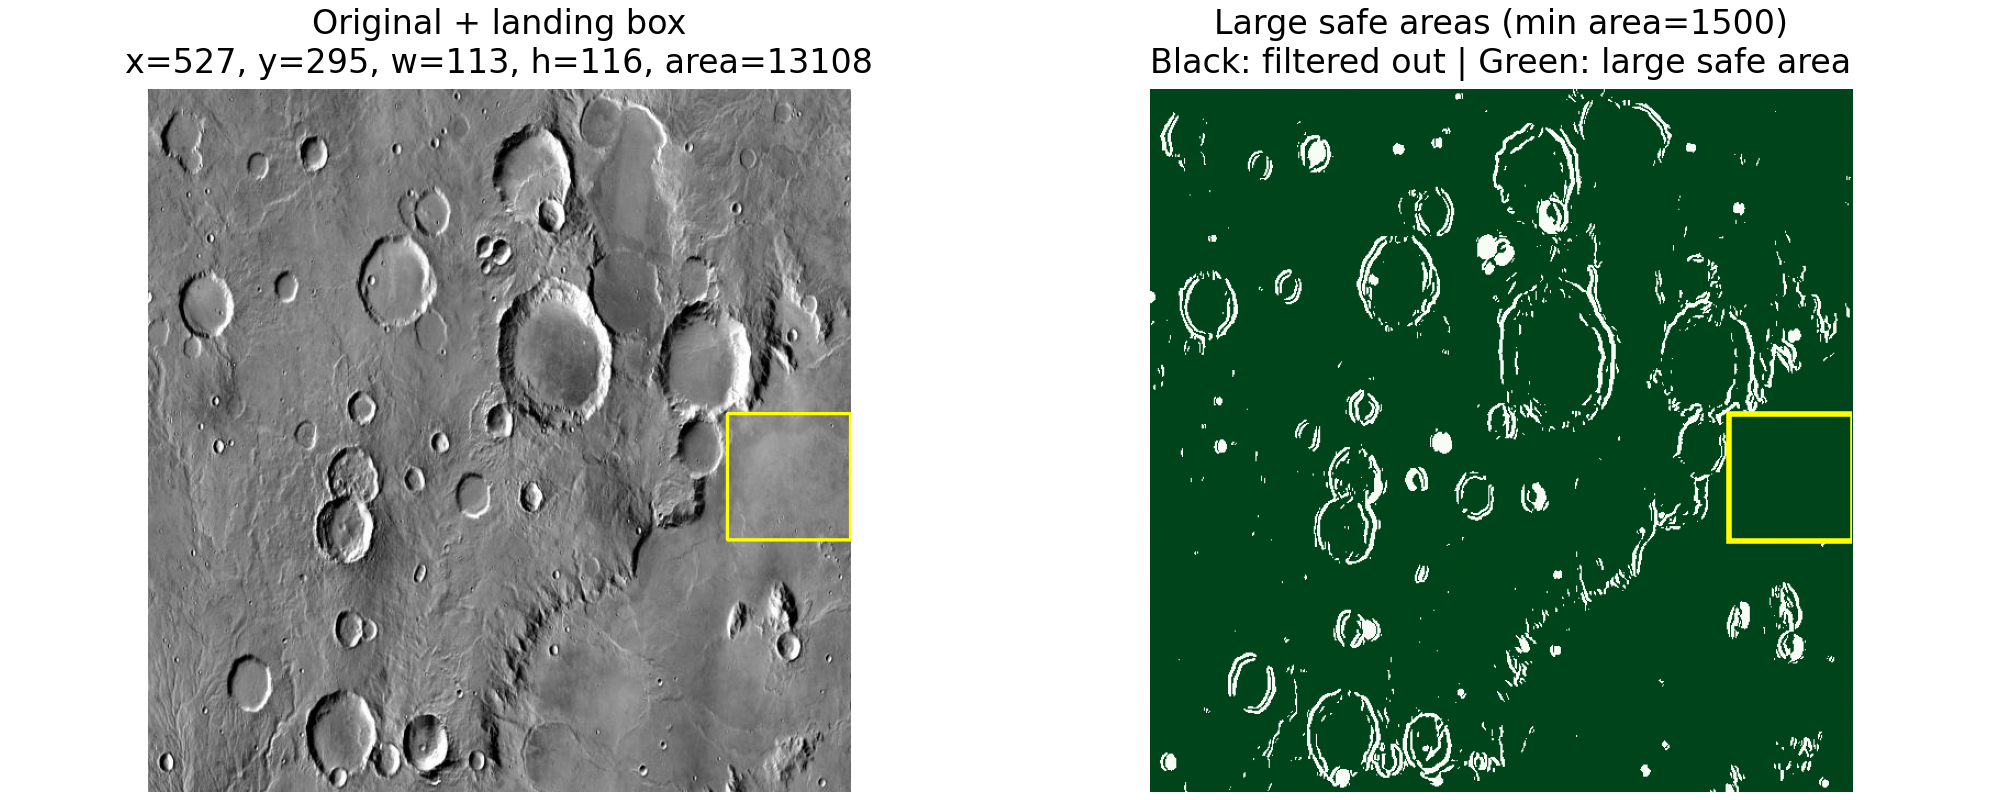
\includegraphics[width=0.8\textwidth]{media/1_1_large_safe_areas.png}
  \caption{Results on crater terrain. The yellow box indicates the largest contiguous safe landing zone. Crater rims are avoided, though well-lit crater interiors remain untriggered by the shadow mask.}
  \label{fig:results_crater}
\end{figure}

\begin{figure}[htbp]
  \centering
  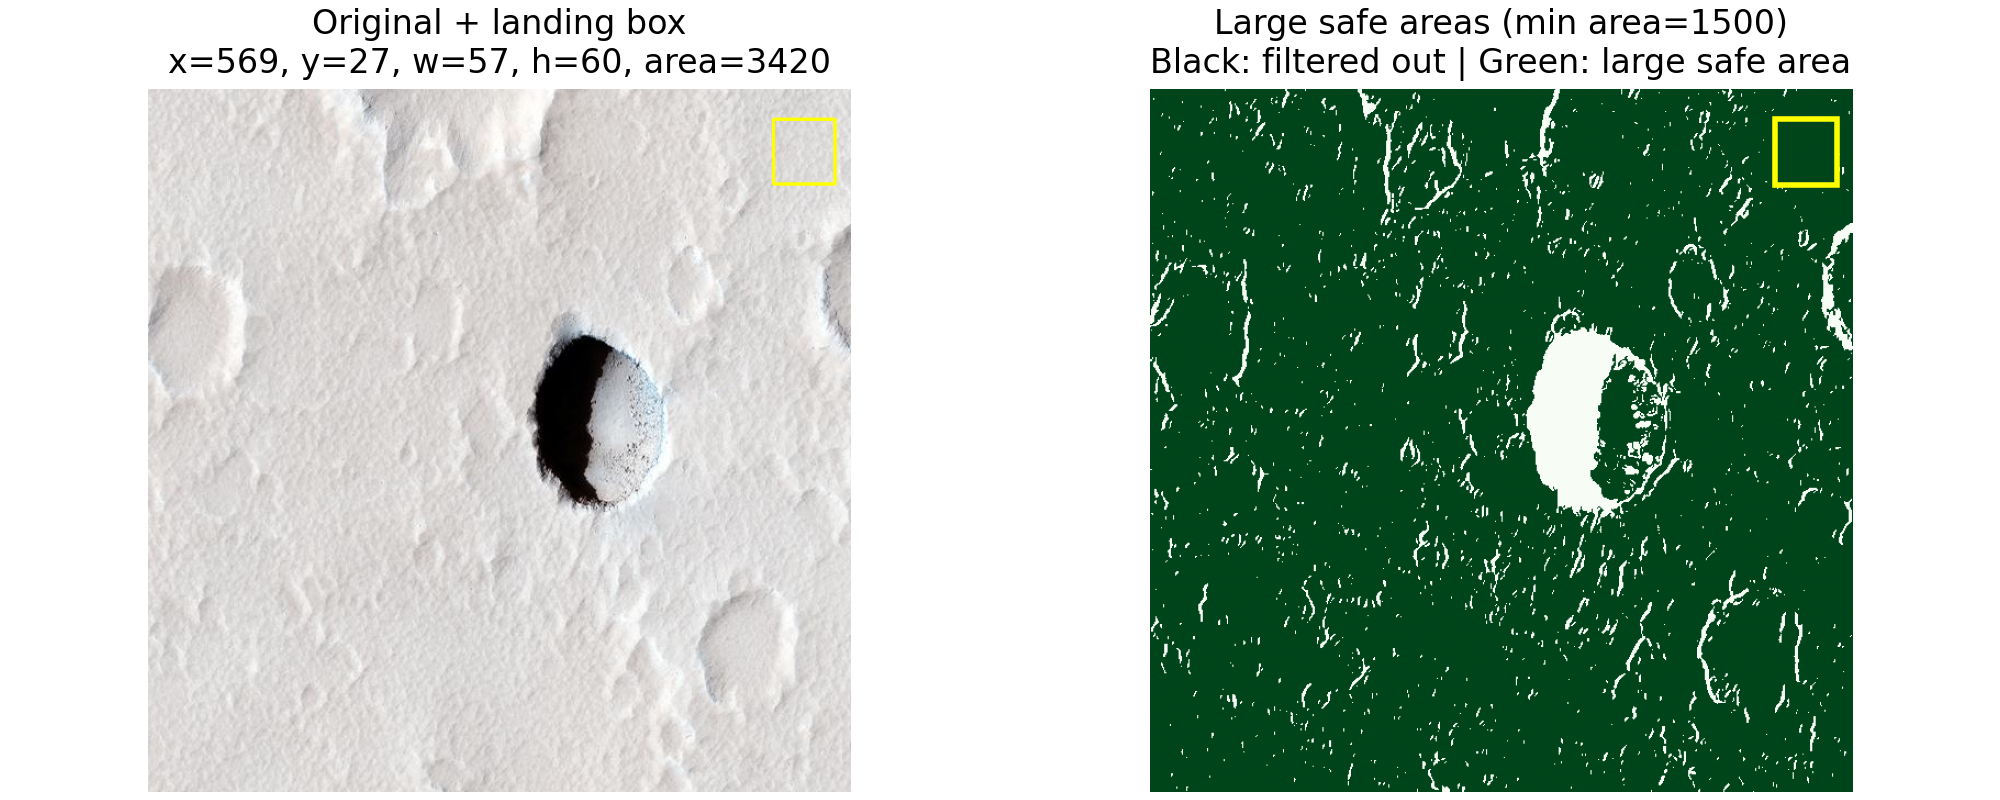
\includegraphics[width=0.8\textwidth]{media/2_2_large_safe_areas.png}
  \caption{Results on rocky terrain. The system avoids rough features and selects a smooth, low-texture surface. The yellow box is constrained by surrounding scattered hazards.}
  \label{fig:results_rocky}
\end{figure}

\begin{figure}[htbp]
  \centering
  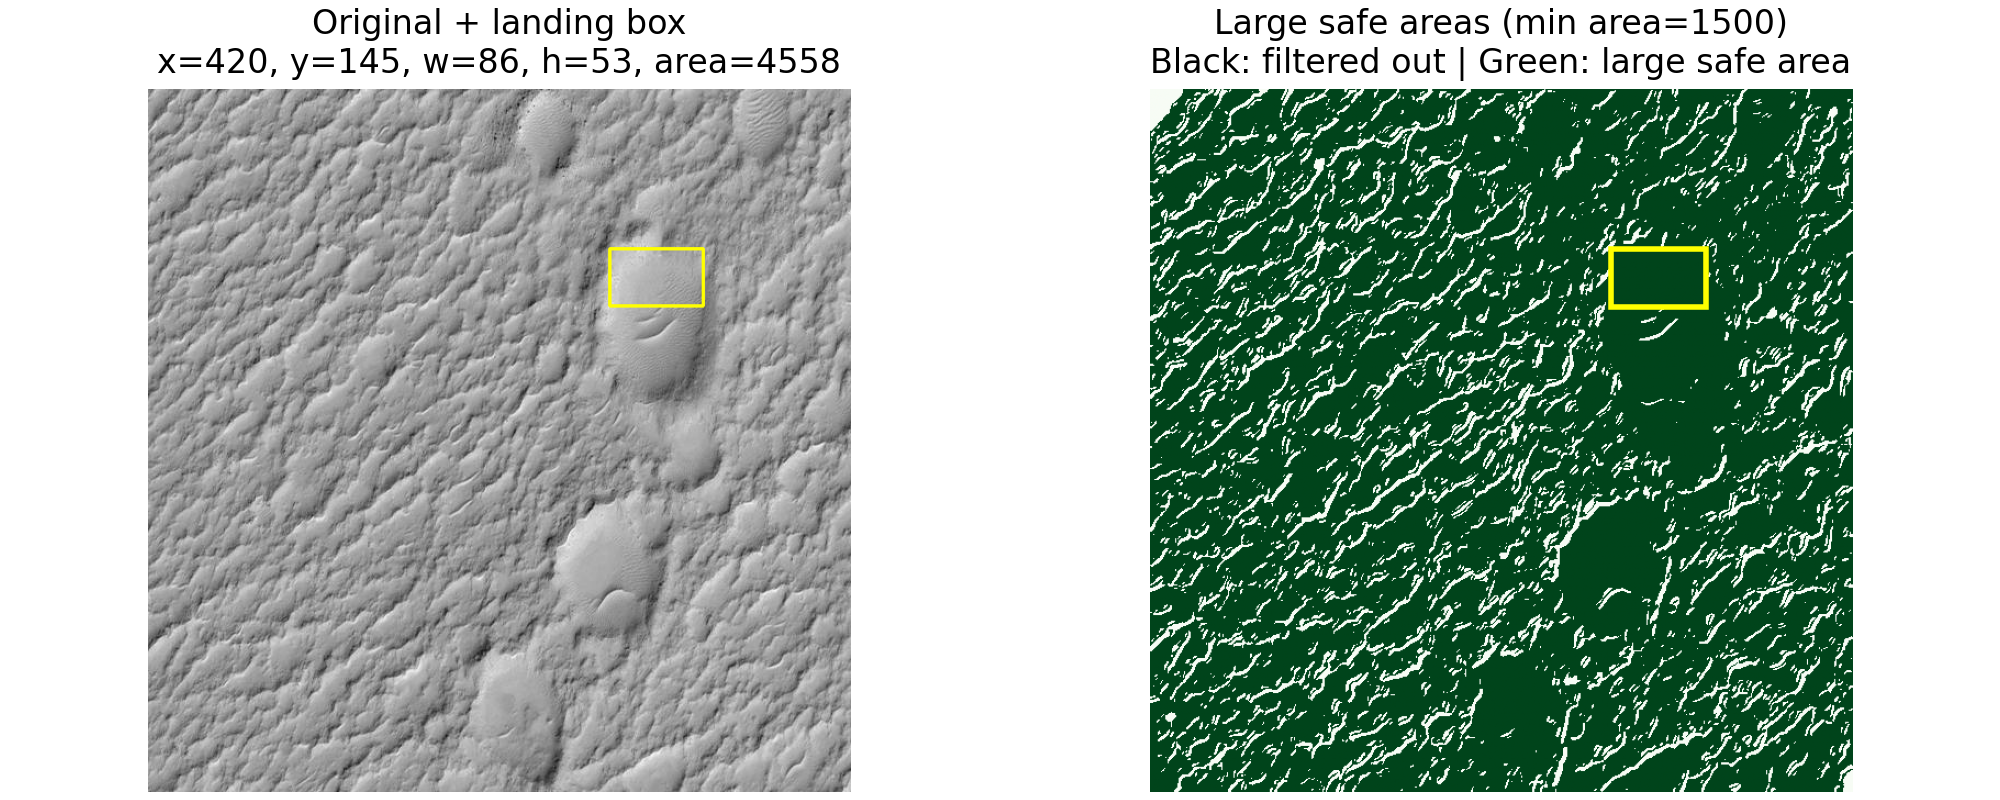
\includegraphics[width=0.8\textwidth]{media/3_3_large_safe_areas.png}
  \caption{Results near a small crater rim. The safe zone is located, but the yellow box is placed directly adjacent to the hazard, illustrating the need for a proximity penalty.}
  \label{fig:results_cliff}
\end{figure}

\section{Limitations and Future Directions}
As a proof-of-concept system, several design choices in this pipeline are intentionally simplified and represent known directions for improvement. The following subsections describe the primary limitations and the most concrete paths to addressing them.
 
\subsection{Thresholding and Proximity Penalties}
All thresholds in the pipeline, such as the fixed intensity threshold $\tau = 40$ used for shadow detection, were selected through manual visual inspection. Fixed thresholds may perform inconsistently under varying solar incidence angles and across landing sites with different surface albedo characteristics. Replacing the fixed threshold with an adaptive scheme, for example, Contrast Limited Adaptive Histogram Equalization (CLAHE) followed by Otsu's thresholding \cite{otsu1979}, would substantially reduce sensitivity to illumination variation. Furthermore, the pipeline currently does not penalize landing zones that are geometrically safe but adjacent to hazardous terrain. Incorporating a distance transform applied to the binary hazard mask into the composite safe score would safely bias the landing zone selection away from hazard boundaries, such as crater rims.

\subsection{Quantitative Benchmarking}
The evaluation in this work is limited to qualitative visual inspection. Quantitative evaluation on a benchmark dataset with expert-annotated safe and unsafe zones derived from rover telemetry or geologist review would enable objective measurement of precision, recall, F1-score, and area under the ROC curve. Developing such a benchmark dataset, potentially by annotating existing high-resolution imagery from the HiRISE instrument \cite{mcewen2007hirise} or by simulation using Mars Digital Terrain Models, is an important direction for future work.

\section{Conclusion}
This paper presented a classical, deterministic computer
vision pipeline for identifying safe landing zones on Mars
from high-resolution descent-like imagery. By fusing Sobel-based
gradient hazard scoring, contour-based shadow augmentation,
and an FFT-based texture-energy score, the pipeline
produces a per-pixel safety map from which the largest viable
landing rectangle is extracted via a maximal-rectangle algorithm \cite{vandevoorde1996maximal}. Qualitative evaluation on crater, rocky-surface, and crater rim
terrain showed that the system can avoid major
hazards such as crater rims and deep shadowed depressions,
while also revealing a limitation regarding hazard proximity without explicit distance penalties. Because the pipeline relies
on no training data and uses only lightweight, deterministic
operations, it offers a potential lightweight alternative for deployment
on radiation-hardened flight processors, where memory and
compute budgets can be challenging for deep learning-based approaches to accommodate.

\section*{Acknowledgments}
The authors acknowledge the Indian Institute of Technology, Gandhinagar, for providing the infrastructure and resources that supported this work.

%Bibliography
\bibliographystyle{unsrt}  
\bibliography{references}  


\end{document}
